    \documentclass[12pt,a4paper]{article}
    \usepackage[T2A]{fontenc}
    \usepackage[utf8]{inputenc}
    \usepackage[russian]{babel}
    \usepackage{amsmath}
    \usepackage{amssymb}
    \usepackage{graphicx}
    \usepackage{floatrow}
    \usepackage{booktabs}
    \usepackage{wrapfig}
    \usepackage{lipsum}
    \usepackage{subcaption}
    \usepackage{fancyhdr}
    \usepackage{mathrsfs}
    \usepackage{tikz}

    \usepackage{graphicx, scalerel}
    \usepackage[warn]{mathtext}
    \usepackage{indentfirst}
    \usepackage[margin = 25mm]{geometry}
    \usepackage{caption}
    \usepackage{multirow}
    \usepackage{gensymb}
    
    \newcommand{\figref}[1]{(См. рис. \ref{#1})}
    \newcommand{\secref}[1]{(См. раздел. \ref{#1})}
    
    \newcommand{\e}[1]{\text{$\cdot10^{#1}$}}
    
    \pagestyle{fancy}
    \fancyhead{}
    \fancyhead[L]{Работа 5.2.1}
    \fancyhead[R]{}
    \fancyfoot[C]{\thepage}
    
    \author{\normalsize Выполнил: Голубович Тимур, группа Б01-110 \\
    	\normalsize 04.10.2023}
    \date{}

    \usepackage{float}
    \restylefloat{table}
    \title{
    	\large Отчет о выполнении лабораторной работы 5.2.1 \\
    	\Large Опыт Франка-Герца
     }

    \begin{document}
    	\maketitle

    \section*{Цель работы}

    Методом электронного возбуждения измерить энергию первого уровня атома гелия в динамическом и статическом режимах.

    \section*{Оборудование и приборы}

    Осциллограф; вольтметр; миллиамперметр; блок источников питания; газонаполненная лампа.
	
    \section*{Теоретическое введение}

    \begin{figure}[h!]
		\centering
		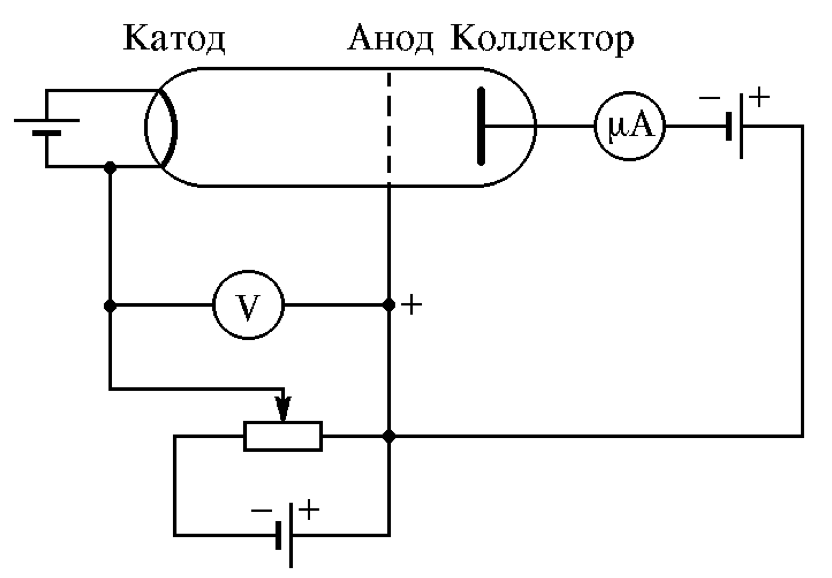
\includegraphics[width=10cm]{res/scheme.png}
		\caption{Схема опыта Франка и Герца}
		\label{Experiment}
	\end{figure}
	
	Одним из простых опытов, подтверждающих существование дискретных уровней энергии атомов, является эксперимент, известный под названием опыта Франка и Герца. Схема опыта изображена на рис. \ref{Experiment}.
	
	Разреженный одноатомный газ (в нашем случае — гелий) заполняет трехэлектродную лампу. Электроны, испускаемые разогретым катодом, ускоряются в постоянном электрическом поле, созданном между катодом и сетчатым анодом лампы и сталкиваются с атомами гелия. Если энергия электрона, налетающего на атом, недостаточна для того, чтобы перевести его в возбужденное состояние, то возможны только упругие соударения.
	
	По мере увеличения разности потенциалов между анодом и катодом энергия электронов увеличивается и, в конце концов, оказывается достаточной для возбуждения атомов. При таких -- неупругих -- столкновениях кинетическая энергия налетающего электрона передается одному из атомных электронов, вызывая его переход на свободный энергетический уровень (возбуждение) или совсем отрывая его от атома (ионизация).
	
	Ток коллектора, пропорциональный числу электронов, попадающих на него за секунду, измеряется микроамперметром.

	При увеличении потенциала анода ток в лампе вначале растет. Однако, когда энергия электронов становится достаточной для возбуждения атомов, ток коллектора резко уменьшается. При дальнейшем увеличении потенциала анода ток коллектора вновь возрастает.

	Следующее замедление роста тока происходит в момент, когда часть
	электронов неупруго сталкивается с атомами два раза: первый раз посередине пути, второй -- у анода и т. д. Таким образом, на кривой зависимости тока коллектора от напряжения анода имеется ряд максимумов и минимумов, отстоящих друг от друга на равные расстояния $\Delta V$. Эти расстояния равны энергии первого возбужденного состояния.
	
 
	\section*{Экспериментальная установка}

    \begin{figure}[h!]
		\centering
		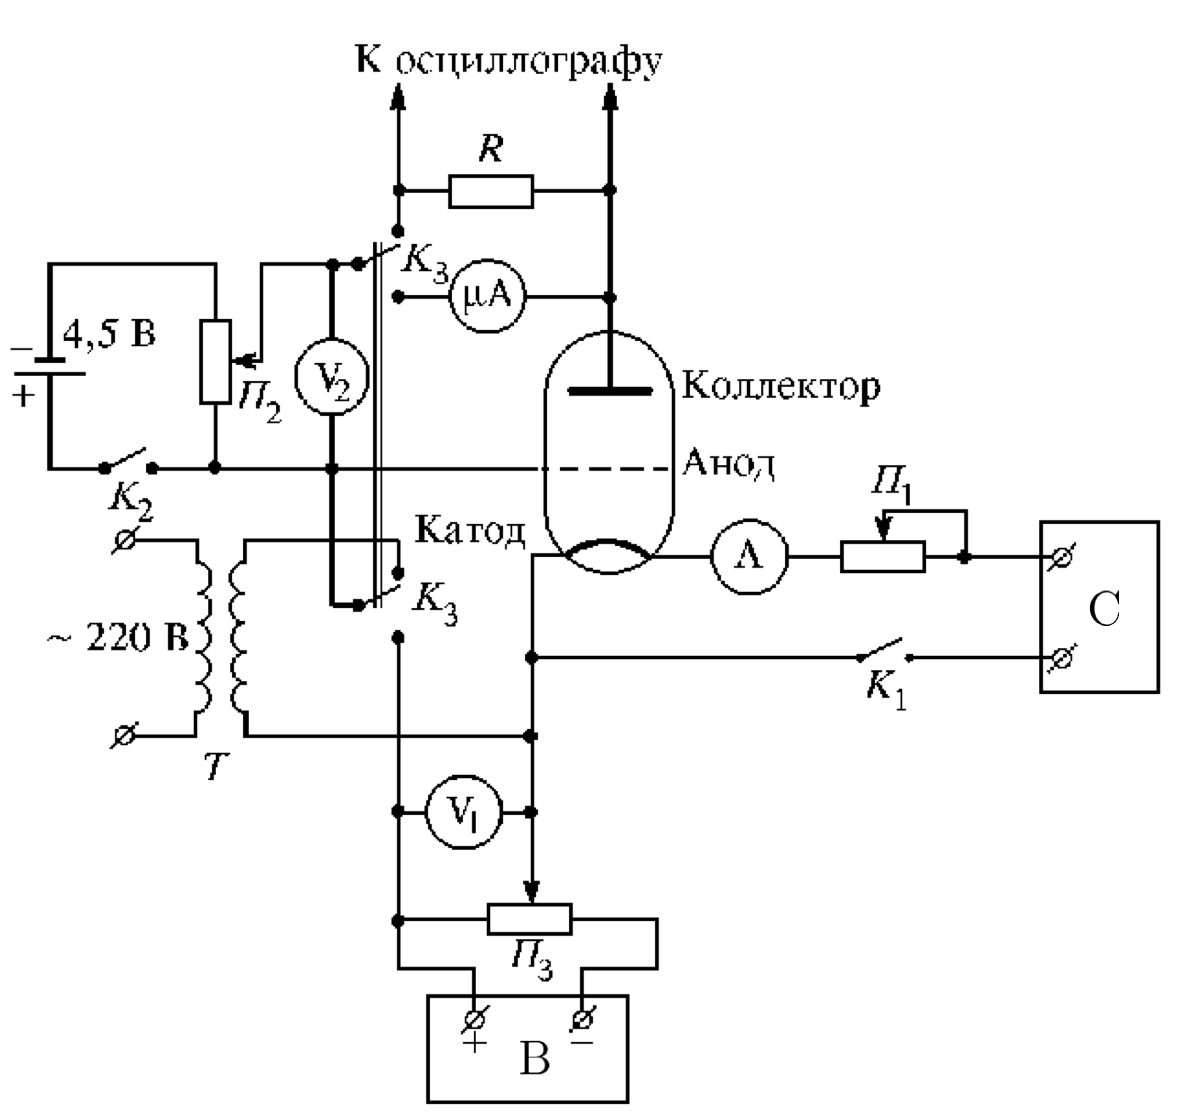
\includegraphics[width=10cm]{res/circuit.png}
		\caption{Схема экспериментальной установки}
		\label{Circuit}
	\end{figure}
	
	Схема экспериментальной установки изображена на рис. \ref{Circuit}. Для опыта используется серийная лампа ионизационного манометра ЛМ-2, заполненная гелием. Напряжение накала подается от стабилизированного источника питания Б7-4. Ток накала контролируется амперметром А. Источник Б7-4 включается в цепь тумблером К$_1$.
	
	В качестве анода используется двойная спираль, окружающая катод. Роль коллектора играет полый металлический цилиндр, соосный с катодом и анодом.
	
	Ускоряющее напряжение подается на анод от выпрямителя Б5-10. Величина этого напряжения регулируется потенциометром П$_3$ и измеряется вольтметром $V_1$. Источник задерживающего потенциала -- батарея КБСЛ (4,5 В) -- включается ключом K$_2$, величина потенциала регулируется потенциометром П$_2$ и измеряется вольтметром $V_2$. Ток в цепи коллектора регистрируется микроамперметром.

	Схему можно переключать из статического режима измерений в динамический режим с помощью ключа K$_3$. На рис. \ref{Circuit} две части сдвоенного ключа K$_3$ изображены отдельно. При динамическом режиме работы ускоряющий потенциал подается с понижающего трансформатора $T$ (220/50 В), а ток коллектора регистрируется осциллографом, подключенным к нагрузочному резистору $R$. Осциллограф следует синхронизировать от сети 50 Гц.

	При определении энергии электронов по разности потенциалов между анодом и катодом следует иметь в виду, что из-за контактной разности потенциалов между катодом и анодом первый максимум не соответствует потенциалу первого возбужденного уровня. Однако контактная разность потенциалов так сдвигает все максимумы, что расстояние между ними не меняется.
 
    \section*{Ход работы}
	
    \begin{enumerate}

        \item Проследим за ходом ВАХ при изменении ускоряющего напряжения для различных задерживающих напряжениях (рис. \ref{Dynamic4}, \ref{Dynamic6} и \ref{Dynamic8}).

        \begin{figure}[h!]
 			\centering
 			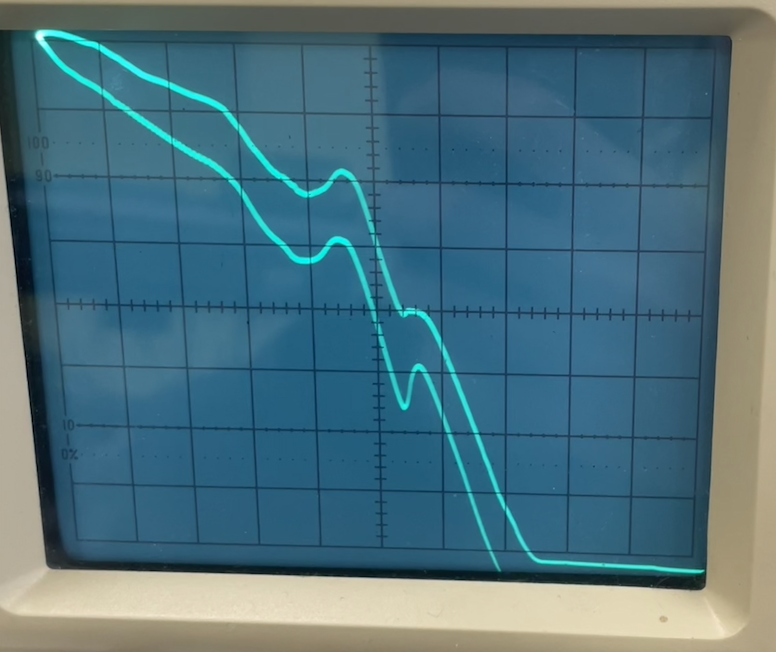
\includegraphics[width=10cm]{src/uno.png}
 			\caption{ВАХ на экране осциллографа при $V_\text{з} = 4 \text{В}$}
            \label{Dynamic4}
 		\end{figure}

        \begin{figure}[h!]
 			\centering
 			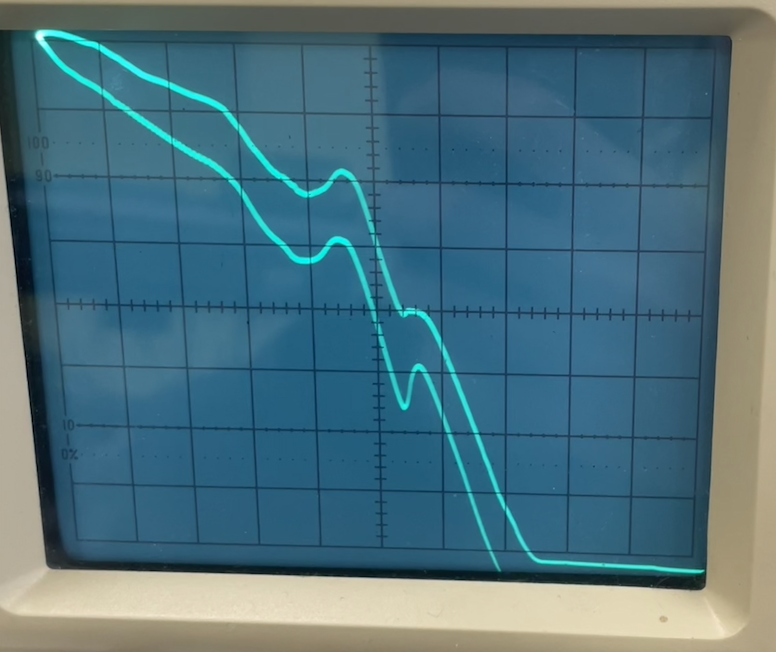
\includegraphics[width=10cm]{src/uno.png}
 			\caption{ВАХ на экране осциллографа при $V_\text{з} = 6 \text{В}$}
            \label{Dynamic6}
 		\end{figure}

        \begin{figure}[h!]
 			\centering
 			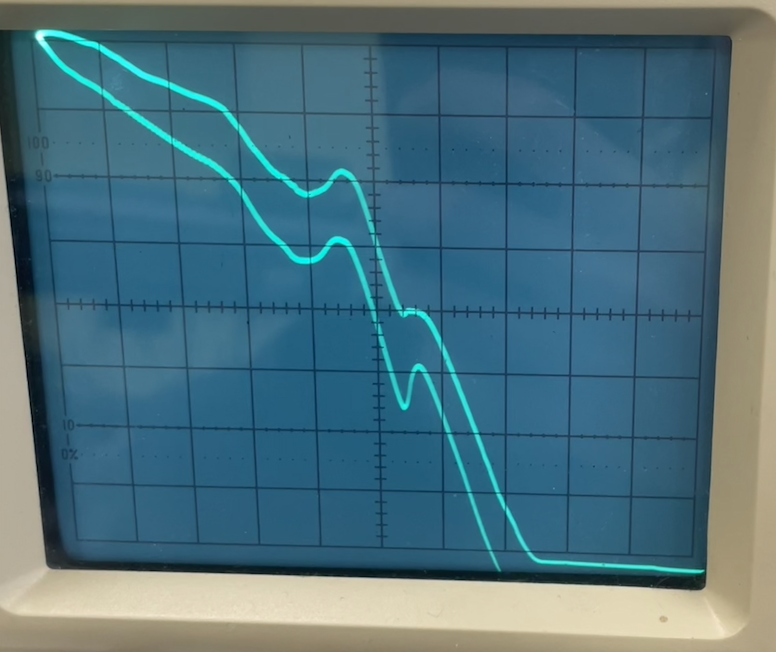
\includegraphics[width=10cm]{src/uno.png}
 			\caption{ВАХ на экране осциллографа при $V_\text{з} = 6 \text{В}$}
            \label{Dynamic8}
 		\end{figure}

        \item При максимальном ускоряющем напряжении измерим на экране расстояния между максимума и минимумами осциллограммы. Проведем такие измерения для 3-х значений задерживающего напряжения: 4, 6 и 8 В. Результаты пишем в таблицу \ref{MaxMin}.

        \item Снимем зависимость коллекторного тока от анодного напряжения $I_\text{к} = f(V_a)$ для 3-х различных значений задерживающего напряжения $V_2 = 4, \; 6, \; 8$ В. Результаты занесем в таблицу \ref{Static}.
         		
		\item По расстоянию между соседними максимумами на осциллограммах определим энергию возбуждения первого уровня атома гелия.
 		
        \begin{table}[h!]
           \centering
           \footnotesize
           \begin{tabular}{c|c|c}
\toprule
$V_\text{з}$, В & $\Delta V_{max}$, В & $\Delta V_{min}$, В \\
\midrule
4 & 14 & 14 \\
6 & 15 & 14 \\
8 & 15 & 14 \\
\bottomrule
\end{tabular}

           \caption{Расстояние между максимумами и расстояние между минимумами в динамическом режиме. Погрешность измерения каждого напряжения $\sigma_V = 1 $ В}
           \label{MaxMin}
        \end{table}

 		Тогда среднее значение:
 		
 		\begin{equation*}
 			\Delta V = (15.0 \pm 3.5) \text{ В} \hspace{20mm} (\text{погрешность}\thicksim 23 \% )
 		\end{equation*}
 	
 		То есть энергия возбуждения первого уровня атома гелия:
 		\begin{equation*}
 			E_1 = (15.0 \pm 3.5) \text{ эВ} \hspace{20mm} (\text{погрешность}\thicksim 23 \% )
 		\end{equation*}
 		
 		
 		\item По результатам таблицы \ref{Static} построим графики зависимостей $I_\text{к} = f(V_a)$ для трех значений задерживающего напряжения.

        \begin{table}[h!]
           \centering
           \footnotesize
           \begin{tabular}{c|ccc}
\toprule
$V_\text{а}$, В & \multicolumn{3}{c}{$I_\text{к}$, мкА } \\
& $V_\text{з} = 4 \text{В}$ & $V_\text{з} = 6 \text{В}$ & $V_\text{з} = 6 \text{В}$ \\
\midrule
 5.0200 & 0.0924 & 0.0562 & 0.0182 \\
15.0300 & 0.3323 & 0.2887 & 0.2403 \\
19.8800 & 0.4439 & 0.3987 & 0.3604 \\
22.9700 & 0.4691 & 0.4352 & 0.4039 \\
23.9200 & 0.3953 & 0.4390 & 0.4093 \\
24.8600 & 0.3914 & 0.2862 & 0.4105 \\
26.1300 & 0.4275 & 0.2720 & 0.1785 \\
31.9000 & 0.6050 & 0.4609 & 0.3226 \\
38.0200 & 0.7014 & 0.5720 & 0.4498 \\
39.0400 & 0.6960 & 0.5714 & 0.4520 \\
40.0600 & 0.6837 & 0.5580 & 0.4430 \\
49.7400 & 0.6894 & 0.5059 & 0.3501 \\
55.1000 & 0.7367 & 0.5443 & 0.3750 \\
60.0800 & 0.7856 & 0.5862 & 0.4189 \\
63.2700 & 0.7988 & 0.5983 & 0.4260 \\
65.3600 & 0.8089 & 0.6008 & 0.4238 \\
71.2000 & 0.8228 & 0.6021 & 0.4151 \\
\bottomrule
\end{tabular}

           \caption{ВАХ для значений задерживающего напряжения 4, 6 и 8 В}
           \label{Static}
        \end{table}

 		\begin{figure}[h!]
 			\centering
 			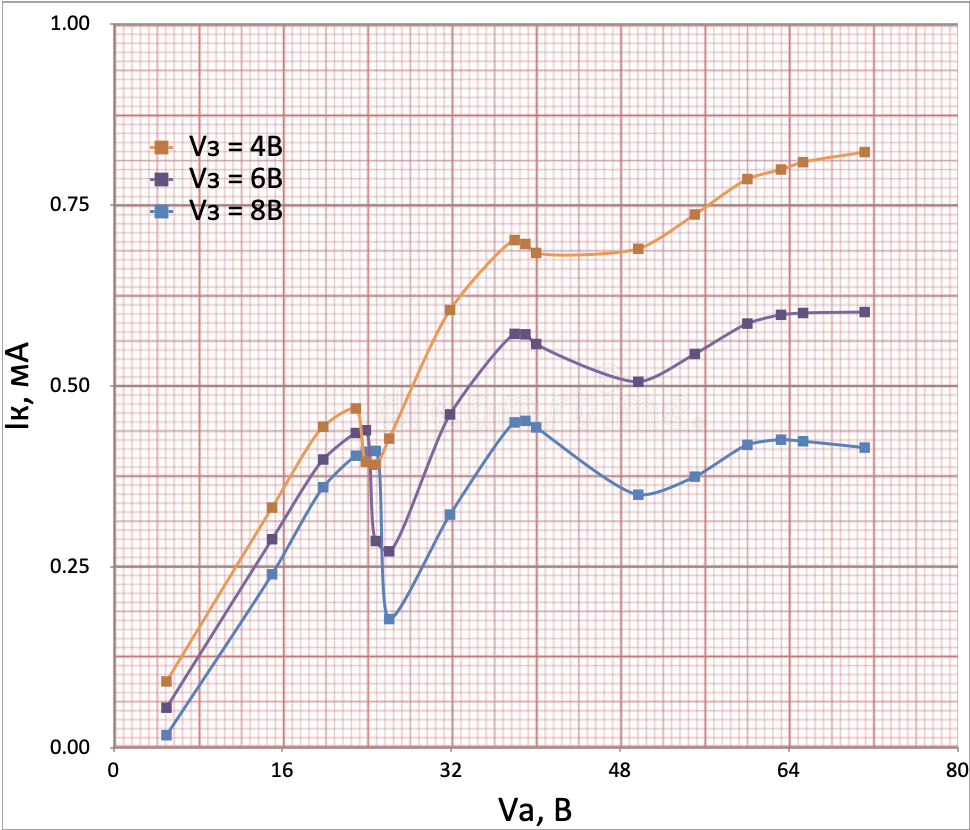
\includegraphics[width=12cm]{src/I_U.png}
 			\caption{Зависимость $I_\text{к}(V_a)$ при различных задерживающих напряжениях}
 		\end{figure}
 	
 		По графику $V_\text{з} = 4 \text{В}$ находим:
 		\begin{equation*}
 			\Delta V = (21.9 \pm 0.2) \text{ В}
 			\hspace{20mm} (\text{погрешность}\thicksim 0.8 \% )
 		\end{equation*}
 	
 		По $V_\text{з} = 6 \text{В}$:
 		\begin{equation*}
 			\Delta V = (22.0 \pm 0.2) \text{ В}
 			\hspace{20mm} (\text{погрешность}\thicksim 0.9 \% )
 		\end{equation*}

        А для $V_\text{з} = 6 \text{В}$:
        \begin{equation*}
 			\Delta V = (21.7 \pm 0.2) \text{ В}
 			\hspace{20mm} (\text{погрешность}\thicksim 0.9 \% )
 		\end{equation*}
 	
 		Такая высокая точность достигается благодаря вольтметру и амперметру, которые в данном случае имеют погрешности 0.01 В и 1 мкА соответственно.
 	
 		И если посчитать среднее значение по этим трем графикам, то получим:
 		\begin{equation*}
 			\boxed{\Delta V^\Sigma = (21.9 \pm 0.3) \text{ В}}
 		\end{equation*}
 	
 		А значит, энергия возбуждения первого уровня атома гелия равна:
 		\begin{equation*}
 			\boxed{E_1^\Sigma = (21.9 \pm 0,3) \text{ эВ}}
 		\end{equation*}
 	
 		Погрешность составляет $\thicksim 1.4 \%$.
 		
 		\item В итоге мы наблюдаем такую картину: значения, полученные при динамическом и статическом методах достаточно сильно разнятся. Однако и погрешность у динамического метода велика -- около 23\%. Статический метод оказался гораздо лучше в плане точности -- его погрешности порядка всего лишь процента.
 		
 		Вдобавок, значение, вычисленное при статическом методе, оказывается чрезвычайно близко к табличному значению в 21.6 эВ, что даже укладывается в полученный интервал для $E_1$.
 	
 	\end{enumerate}

    \newpage
    
	\section*{Вывод}
 
    В данной работе мы воспроизвели опыт Франка-Герца, который подтверждает наличие дискретных уровней возбуждения атомов. Опыт был проведен в динамическом и статическом режимах, из которых были получены следующие результаты для энергии возбуждения первого уровня атома гелия:

 	\begin{itemize}
 		\item $E_\text{dynamic} = (15.0 \pm 3.5) \text{ эВ} \hspace{20mm} (\text{погрешность}\thicksim 23 \% )$
 		
 		\item $E_\text{static} \;\;\; = (21.9 \pm 0.3) \text{ эВ} \hspace{20mm} (\text{погрешность}\thicksim 1.4 \% )$
 	\end{itemize}

 	Причем табличное значение $E = 21.6$ эВ. Как видим, статический метод дает очень близкое к нему значение и даже в пределах погрешностей совпадает. Динамический метод имеет куда большую ошибку, а также дает результат, находящийся гораздо дальше от табличного.
 	
 	Ошибка динамического метода связана с несовершенством техники измерения. Погрешности при статическом методе все же имеют куда меньшие значения благодаря точности вольтметра и амперметра. В контексте этой работы, процентаж ошибки этих приборов составляет всего лишь $\thicksim 0.1-3.0\%$.

    \vfill

    \begin{thebibliography}{9}
    	\bibitem{max} \emph{Лабораторный практикум по общей физике. В 3 томах. Том 3. Квантовая физика: учебное пособие} под ред. Ю. М. Ципенюка
    \end{thebibliography}

\end{document}
